\documentclass[11pt,a4paper,twoside]{tesis}
% SI NO PENSAS IMPRIMIRLO EN FORMATO LIBRO PODES USAR
%\documentclass[11pt,a4paper]{tesis}

\usepackage{graphicx}
\graphicspath{ {images/} }
\usepackage[utf8]{inputenc}
\usepackage[spanish]{babel}
\usepackage[left=3cm,right=3cm,bottom=3.5cm,top=3.5cm]{geometry}
\usepackage{amsthm}
\usepackage{amsmath}
\usepackage{amssymb}
\usepackage[T1]{fontenc}
\newtheorem{exmp}{Ejemplo}
\usepackage[titlenumbered,ruled]{algorithm2e}

\newcommand{\ch}{\textit{chase}}

\begin{document}


%%%% CARATULA

\def\autor{Pablo Víctor Fromer}
\def\tituloTesis{Datalog +/-, \vspace{.2cm} \\ una interfaz tolerante a la inconsistencia }
\def\runtitulo{Datalog +/-, una interfaz tolerante a la inconsistencia}
\def\runtitle{Datalog +/-, una interfaz tolerante a la inconsistencia}
\def\director{María Vanina Martinez}
\def\codirector{Ricardo Oscar Rodriguez}
\def\lugar{Buenos Aires, 2019}
\newcommand{\HRule}{\rule{\linewidth}{0.2mm}}
%
\thispagestyle{empty}

\begin{center}\leavevmode

\vspace{-2cm}

\begin{tabular}{l}

\includegraphics[width=2.6cm]{logofcen.pdf}
\end{tabular}


{\large \sc Universidad de Buenos Aires

Facultad de Ciencias Exactas y Naturales

Departamento de Computaci\'on}

\vspace{6.0cm}

%\vspace{3.0cm}
%{
%\Large \color{red}
%\begin{tabular}{|p{2cm}cp{2cm}|}
%\hline
%& Pre-Final Version: \today &\\
%\hline
%\end{tabular}
%}
%\vspace{2.5cm}

\begin{huge}
\textbf{\tituloTesis}
\end{huge}

\vspace{2cm}

{\large Tesis de Licenciatura en Ciencias de la Computaci\'on}

\vspace{2cm}

{\Large \autor}

\end{center}

\vfill

{\large

{Director: \director}

\vspace{.2cm}

{Codirector: \codirector}

\vspace{.2cm}

\lugar
}

\newpage\thispagestyle{empty}


%%%% ABSTRACTS, AGRADECIMIENTOS Y DEDICATORIA
%\frontmatter
%\pagestyle{empty}
%%\begin{center}
%\large \bf \runtitulo
%\end{center}
%\vspace{1cm}
\chapter*{\runtitulo}

\noindent La princesa Leia, líder del movimiento rebelde que desea reinstaurar la República en la galaxia en los tiempos ominosos del Imperio, es capturada por las malévolas Fuerzas Imperiales, capitaneadas por el implacable Darth Vader. El intrépido Luke Skywalker, ayudado por Han Solo, capitán de la nave espacial ``El Halcón Milenario'', y los androides, R2D2 y C3PO, serán los encargados de luchar contra el enemigo y rescatar a la princesa para volver a instaurar la justicia en el seno de la Galaxia (aprox. 200 palabras).

\bigskip

\noindent\textbf{Palabras claves:} Guerra, Rebelión, Wookie, Jedi, Fuerza, Imperio (no menos de 5).

%\cleardoublepage
%%\begin{center}
%\large \bf \runtitle
%\end{center}
%\vspace{1cm}
\chapter*{\runtitle}

\noindent In a galaxy far, far away, a psychopathic emperor and his most trusted servant -- a former Jedi Knight known as Darth Vader -- are ruling a universe with fear. They have built a horrifying weapon known as the Death Star, a giant battle station capable of annihilating a world in less than a second. When the Death Star's master plans are captured by the fledgling Rebel Alliance, Vader starts a pursuit of the ship carrying them. A young dissident Senator, Leia Organa, is aboard the ship \& puts the plans into a maintenance robot named R2-D2. Although she is captured, the Death Star plans cannot be found, as R2 \& his companion, a tall robot named C-3PO, have escaped to the desert world of Tatooine below. Through a series of mishaps, the robots end up in the hands of a farm boy named Luke Skywalker, who lives with his Uncle Owen \& Aunt Beru. Owen \& Beru are viciously murdered by the Empire's stormtroopers who are trying to recover the plans, and Luke \& the robots meet with former Jedi Knight Obi-Wan Kenobi to try to return the plans to Leia Organa's home, Alderaan. After contracting a pilot named Han Solo \& his Wookiee companion Chewbacca, they escape an Imperial blockade. But when they reach Alderaan's coordinates, they find it destroyed - by the Death Star. They soon find themselves caught in a tractor beam \& pulled into the Death Star. Although they rescue Leia Organa from the Death Star after a series of narrow escapes, Kenobi becomes one with the Force after being killed by his former pupil - Darth Vader. They reach the Alliance's base on Yavin's fourth moon, but the Imperials are in hot pursuit with the Death Star, and plan to annihilate the Rebel base. The Rebels must quickly find a way to eliminate the Death Star before it destroys them as it did Alderaan (aprox. 200 palabras).

\bigskip

\noindent\textbf{Keywords:} War, Rebellion, Wookie, Jedi, The Force, Empire (no menos de 5). % OPCIONAL: comentar si no se quiere

%\cleardoublepage
%\chapter*{Agradecimientos}

\noindent Lorem ipsum dolor sit amet, consectetur adipiscing elit. Fusce sapien ipsum, aliquet eget convallis at, adipiscing non odio. Donec porttitor tincidunt cursus. In tellus dui, varius sed scelerisque faucibus, sagittis non magna. Vestibulum ante ipsum primis in faucibus orci luctus et ultrices posuere cubilia Curae; Mauris et luctus justo. Class aptent taciti sociosqu ad litora torquent per conubia nostra, per inceptos himenaeos. Mauris sit amet purus massa, sed sodales justo. Mauris id mi sed orci porttitor dictum. Donec vitae mi non leo consectetur tempus vel et sapien. Curabitur enim quam, sollicitudin id iaculis id, congue euismod diam. Sed in eros nec urna lacinia porttitor ut vitae nulla. Ut mattis, erat et laoreet feugiat, lacus urna hendrerit nisi, at tincidunt dui justo at felis. Class aptent taciti sociosqu ad litora torquent per conubia nostra, per inceptos himenaeos. Ut iaculis euismod magna et consequat. Mauris eu augue in ipsum elementum dictum. Sed accumsan, velit vel vehicula dignissim, nibh tellus consequat metus, vel fringilla neque dolor in dolor. Aliquam ac justo ut lectus iaculis pharetra vitae sed turpis. Aliquam pulvinar lorem vel ipsum auctor et hendrerit nisl molestie. Donec id felis nec ante placerat vehicula. Sed lacus risus, aliquet vel facilisis eu, placerat vitae augue.
 % OPCIONAL: comentar si no se quiere

%\cleardoublepage
%\hfill \textit{A mi persona favorita.}
  % OPCIONAL: comentar si no se quiere

\cleardoublepage
\tableofcontents

\mainmatter
\pagestyle{headings}

%%%% ACA VA EL CONTENIDO DE LA TESIS

\chapter{Introducción}
\section{Motivación Opcion 1}

Los lenguajes ontológicos, los sistemas basados en reglas y sus integraciones han jugado un rol central en el desarrollo de la Web Semántica…  Antes del surgimiento de Datalog +/- no existía literatura que explique cómo generalizar reglas y dependencias de bases de datos de manera que puedan expresar axiomas ontológicos. De esta manera no estaba cubierto el interés en la comunidad de la Web Semántica por conseguir formalismos altamente escalables que pudieran hacer que la red se beneficie de las tecnologías y las optimizaciones ya implementadas en los motores de bases de datos.

Datalog +/- es una serie de variantes del lenguaje Datalog que son particularmente adecuadas para responder consultas sobre ontologías de manera eficiente. Estas variantes extienden Datalog con la posibilidad de cuantificar existencialmente a las variables en las implicaciones de las reglas y otra serie de ventajas, mientras que al mismo tiempo restringen el lenguaje de manera sintáctica con el objetivo de asegurar tratabilidad.

Por otro lado, tanto en el campo de las bases de datos como en el de la Web Semántica es ampliamente reconocido que la inconsistencia es un problema que no puede ser ignorado. Al momento de integrar información proveniente de diversas fuentes, ya sea para popular una ontología o para responder una consulta, las restricciones de integridad son muy propensas a ser violadas en la práctica. En este trabajo proponemos una implementación de la semántica IAR, la cual describe un método para tratar ....

El objetivo de esta tesis es presentar una herramienta... una herramienta que tiene el propósito de acercar a la comunidad una implementación de Datalog+/-, con el objetivo de poder acceder a este lenguaje de manera fácil, a través de Internet...

\section{Datalog +/-}

En esta sección vamos a recordar los elementos principales del lenguaje Datalog tal como se definen en el paper \textit{A General Datalog-Based Framework for
Tractable Query Answering over Ontologies}\cite{JWS}.
Con respecto a los ingredientes elementales, se asumen constantes, nulos y variables de la siguiente manera; estos son los argumentos de las fórmulas atómicas en las bases de datos, consultas y dependencias.
Se asume (i) un universo infinito de constantes  $\Delta$ (las cuáles forman el dominio de la base de  datos), (ii) un conjunto infinito de nulos etiquetados $\Delta_{N}$ (representando valores desconocidos), y (iii) un conjunto infinito de variables X (que se utilizan en las consultas y en las dependencias). Cada constante representa un valor diferente, mientras que nulos distintos podrían representar el mismo valor. 
Se asume un orden lexicográfico en  $\Delta \cup \Delta_{N}$, donde los símbolos de $\Delta_{N}$ siguen a los de $\Delta$. Se denota por $X$ a una sequencia de variables $X_{1}$, ..., $X_{K}$ con $k > 0$.

Se definen las fórmulas atómicas, que ocurren en bases de datos, consultas, y dependencias, y que se construyen en base a los nombres de las relaciones y los términos. Se asume un \textit{esquema relacional $R$}, el cual constituye un conjunto finito de \textit{nombres de relación}, o \textit{símbolos de predicado}. La posición \textit{P[i]} identifica al \textit{i}-esimo argumento de un predicado \textit{P}. Un \textit{término t} es una constante, un nulo o variable. Una \textit{fórmula atómica} (o \textit{átomo}) a tiene la forma \textit{P}($t_{1}$,...,$t_{n}$), donde \textit{P} es un predicado $n$-ario, y $t_{1}$,...,$t_{n}$ son términos. Se denotan por \textit{pred}(a) y \textit{dom}(a) su predicado y al conjunto de sus argumentos, respectivamente. Esta notación se extiende de manera natural para conjuntos y conjunciones de átomos. 

Podemos definir ahora la noción de base de datos relativa a un esquema relacional, junto con la sintaxis y la semántica de las consultas conjuntivas y las consultas conjuntivas booleanas a una base de datos. Una \textit{instancia de base de datos} $D$ para un esquema relacional $R$ es un conjunto de átomos (posiblemente infinito) con predicados de R y argumentos de $\Delta$. Una consulta conjuntiva sobre $R$ tiene la forma $Q(\textbf{X}) = \exists\textbf{Y}\Phi(\textbf{X},\textbf{Y})$, donde $\Phi(\textbf{X},\textbf{Y})$ es una conjunción de átomos con las variables \textbf{X} y \textbf{Y}, y eventualmente constantes, pero sin nulos. Una consulta conjuntiva \textit{Booleana} sobre $R$ es una consulta conjuntiva de la forma $Q() = \exists\textbf{Y}\Phi(\textbf{X},\textbf{Y})$, donde todas las variables están cuantificadas existencialmente. El conjunto de todas las respuestas a una consulta conjuntiva $Q(\textbf{X}) = \exists\textbf{Y}\Phi(\textbf{X},\textbf{Y})$ sobre una base de datos es el conjunto de todas las tuplas \textbf{t} sobre $\Delta$ para las cuales existe un homomorfismo $\mu: \textbf{X} \cup \textbf{X} \rightarrow \Delta \cup \Delta_{N}$ tales que $\mu(\Phi(\textbf{X},\textbf{Y})) \subseteq D$ y $\mu(\textbf{X}) = D$

\begin{exmp}\label{ejemplo_base_d}
Consideremos una base de datos de películas, que guarda información acerca de actores, directores y películas. El esquema relacional $R$ consiste en los predicado unarios \textit{pelicula}, \textit{actor}, \textit{director},  y en los predicados binarios \textit{actuaEn}, \textit{dirigidaPor} y \textit{trabajaronJuntos}.  Una base de datos $D$ para el esquema  $R$ puede estar dada por: 
    \begin{equation}
        $$D = \{\textit{pelicula(``Volver al Futuro''), pelicula(``Esperando la Carroza''), actuaEn(``Esperando la Carroza'', ``Antonio Gasalla''), actuaEn(``Esperando la Carroza'', ``China Zorrilla''),
        actor(``Antonio Gasalla''), dirigidaPor(``Esperando la Carroza'', ``Alejandro Doria'')}\}$$
    \end{equation}

Una posible consulta conjuntiva para esta base de datos podría ser Q(X) = pelicula(X) $\land$ actuaEn(X, Y), que pregunta por todas las películas en las que alguien haya actuado, cuya respuesta es el conjunto de una sola tupla $\{("Esperando la Carroza")\}$;  mientras que un ejemplo de consulta conjuntiva booleana es Q() =  actor(X) $\land$ actuaEn(``Volver al Futuro'', X), la cual pregunta si hay algún actor que haya actuado en Volver al Futuro, cuya respuesta en No.

\end{exmp}



\iffalse
$$D = \{\textit{pelicula(``Esperando la carroza''), pelicula(``Volver al Futuro''), pelicula(``Thelma y Louise''), actuaEn(``Esperando la Carroza'', ``Antonio Gasalla''), actuaEn(``Esperando la Carroza'', ``China Zorrilla''), actuaEn(``Volver al futuro, ``Michael J. Fox''), actuaEn(``Thelma y Louise, ``Susan Sarandon''), actuaEn(``Thelma y Louise'', ``Brad Pitt''), dirigidaPor(``Volver al Futuro'', ``Robert Zemeckis'')}\}$$
\fi



\subsection{Dependencias generadoras de tuplas (TGDs)}
Las dependencias generadoras de tuplas (TGDs) son restricciones sobre una base de datos en la forma general de las reglas de Datalog.....
Dado un esquema relacional $R$, una TGD $\sigma$ es una fórmula de primer orden de la forma $\forall X \forall Y \Phi (X, Y) \rightarrow \exists Z \Psi (X, Z)$, donde $ \Psi (X, Z)$ y $\Phi (X, Y)$ son conjunciones de átomos sobre $R$, llamadas el \textit{cuerpo} y la \textit{cabeza} de $\sigma$, denotadas $cuerpo(\sigma)$ y $cabeza(\sigma)$ respectivamente. Tal $\sigma$ es satisfecha en una base de datos $D$ para $R$ ssi, toda vez que exista un homomorfismo $h$ que mapea los atomos de $\Phi(X, Y)$ a atomos de $D$, existe una extensión $h\prime$ de $h$ que mapea los atomos de $\Psi (X, Z)$ a átomos de $D$. Todos los conjuntos de $TGDs$ son finitos. Usualmente omitimos los cuantificadores universales en las TGDs.
\iffalse
\begin{exmp}
{\rb
    Tomando en cuenta el ejemplo anterior, un posible conjunto de TGDs parar $R$ puede estar dado por $\Sigma = \{\forall X pelicula(X) \rightarrow \exists Z dirigidaPor(X, Z), 
    \forall X \forall Y \forall W actuaEn(X, Y) \land dirigidaPor(X, W) \rightarrow \trabajaronJuntos(Y, W) \}$
    }
\end{exmp}   
\fi


\begin{exmp}\label{ejemplo_tgds}
    Tomando en cuenta el ejemplo anterior, un posible conjunto de TGDs parar $R$ puede estar dado por
\begin{itemize}
    \item Toda película fue dirigida por un director:  $$pelicula(X) \rightarrow \exists Z dirigidaPor(X, Z)$$
    \item Si alguien dirigió una película entonces es un director: $$dirigidaPor(X, Y) \rightarrow director(Y)$$
    \item Si alguien actuó una película entonces es un actor: $$actuaEn(X, Y) \rightarrow actor(Y)$$
    \item Si un actor actuó en una película que fue dirigida por un director, eso implica que el actor y el director trabajaron juntos: $$actuaEn(X, Y) \land dirigidaPor(X, W) \rightarrow trabajaronJuntos(Y, W) $$ 
\end{itemize}

Es simple ver que ninguna de las TGDs anteriores es satisfecha en $D$. Para que esto suceda podemos considerar $D\prime$ que extiene a $D$ de la siguiente manera:

\begin{equation}
    $$ $D\prime$ = D $\cup$ \{\textit{dirigidaPor(``Volver al Futuro'', ``Robert Zemeckis''), director(``Robert Zemeckis''), actor(``China Zorilla''), director(``Alejandro Doria), trabajaronJuntos(``Antonio Gasalla'', ``Alejandro Doria''), trabajaronJuntos(``China Zorilla'', ``Alejandro Doria'')}\}$$
\end{equation} 

Ahora todas las TGDs están satisfechas en $D\prime$.

\end{exmp} 

\subsection{Respondiendo consultas bajo TGDs}

La evaluación de una consulta conjuntiva o una consulta conjuntiva booleana sobre una base de datos bajo un conjunto de TGDs se define como se describre a continuación. Dada una base de datos $D$ para $R$, y un conjunto de TGDs $\Sigma$ sobre $R$, el conjunto de modelos de $D$ y $\Sigma$, el cual denotamos por $mods(D,\Sigma)$, es el conjunto (posiblemente infinito) de todas las bases de datos $B$ tales que (i) $D \subseteq B$ y (ii) toda $\sigma \in \Sigma$ es satisfecha en $B$. El conjunto de todas las respuestas para una consulta conjuntiva $Q$, denotado por $ans(Q, D, \Sigma)$, es el conjunto de todas las tuplas \textbf{a} tales que \textbf{a} $\in Q(B)$ para todo $B \in mods(D, \Sigma)$. La respuesta para una consulta conjuntiva booleana $Q$ a $D$ es \textit{Sí}, denotada por $D \cup \Sigma \models Q$, si solo si, $ans(Q, D, \Sigma) \neq \emptyset$. Notar que responser consultas bajo TGDs para el caso general es indecidible \cite{beeri}, aún cuando el esquema y las TGDs son fijas \cite{cali}. 


\begin{exmp} \label{ejemplo_responder_consultas_bajo_tgds}
Si consideramos la base $D$ del ejemplo \ref{ejemplo_base_d} y las TGDs del ejemplo \ref{ejemplo_tgds} podemos ver que $D \notin mods(D, \Sigma)$ ya que como dijimos antes estas TGDs no se satisfacen en $D$. Por el contrario  $D\prime \in mods(D, \Sigma)$, es decir $D\prime$ es modelo de $D$ y $\Sigma$. En particular las siguientes bases de datos son modelos de  $D$ y $\Sigma$:   

\begin{itemize}
    \item 
      \(D_1\) = D \(\cup\) \{\textit{dirigidaPor(``Volver al Futuro'', ``Steven Spielberg''), director(``Steven Spielberg''),
    actor(``China Zorilla''), director(``Alejandro Doria''), trabajaronJuntos(``Antonio Gasalla'', ``Alejandro Doria''), trabajaronJuntos(``China Zorilla'', ``Alejandro Doria'')}\}
    \item  \(D_2\) = D \(\cup\)  \{\textit{dirigidaPor(``Volver al Futuro'', ``Robert Zemeckis''), director(``Robert Zemeckis''), actuaEn(``Volver al Futuro'', ``Michael J. Fox''), actor(``Michael J. Fox''), trabajaronJuntos(``Michael J. Fox'', ``Robert Zemeckis''),  actor(``China Zorilla''), director(``Alejandro Doria''), trabajaronJuntos(``Antonio Gasalla'', ``Alejandro Doria''), trabajaronJuntos(``China Zorilla'', ``Alejandro Doria'')}\}

\end{itemize} 

Notemos que el átomo \textit{película(Volver al Futuro)} está en todos los \textit{modelos} de $D$ y $\Sigma$, por lo tanto la consulta conjuntiva boleana $Q()$ = película(Volver al Futuro) evalúa a \textit{Sí} en $D$ y $\Sigma$, y lo mismo ocurre con $Q() = trabajaronJuntos(``China Zorrilla", ``Alegandro Doria")$. Por el contrario, la consulta $Q() = dirigidaPor(``Volver al Futuro", ``Robert Zemeckis")$ no es verdadera en todos los \textit{modelos} de $D$ y $\Sigma$, por lo tanto esta consulta evalúa a \textit{No}.
\end{exmp} 

Recordamos que el problema de evaluar una consulta conjuntiva bajo TGDs es LOGSPACE-equivalente al problema de evaluar una consulta conjuntiva booleana [\cite{Chandra}, \cite{Deutsch}, \cite{Fagin}, \cite{Johnson}]. Por eso nos enfocamos aquí solo en el problema de responder consultas conjuntivas booleanas. Recordamos también que responder consultas bajo TGDs es equivalente a responder bajo TGDs que tienen un solo átomo en sus cabezas. Por lo tanto, asumimos sin pérdida de generalidad, que toda TGD tiene un solo átomo en su cabeza.


\subsection{El chase}

El \textit{chase} es un procedimiento para reparar una base de datos con respecto a un conjunto de dependencias, de manera tal que el resultado del chase satisfaga esas dependencias. Por \textit{chase} nos referimos tanto al procedimiento como a su resultado. El TGD chase trabaja sobre una base de datos a través de aplicar las TGDs como se explica a continuación. Considere una base de datos $D$ para un esquema relacional $R$, y una TGD $\sigma$ sobre $R$ de la forma $\Phi (X, Y) \rightarrow \exists Z \Psi (X, Z)$. Entonces, $\sigma$ es \textit{aplicable} a $D$ si existe un homomorfismo \textit{h} que mapee los átomos de $\Phi (X, Y)$ a átomos de $D$. Sea $\sigma$ aplicable a $D$, y sea $h_1$ un homomorfismo que extiende \textit{h} de la siguiente manera: para cada $X_i \in \textbf{X}, h_1(X_i) = h(X_i)$; para cada $Z_j \in \textbf{Z}, h_1(Z_j) = z_j$, siendo $z_j$ un nulo "fresco", es decir, $z_j \in \Delta_N, z_j$ no ocurre en $D$, y $z_j$ sigue lexicográficamente a todos los otros nulos introducidos previamente. Al aplicar $\sigma$ a $D$, se agrega a $D$ el átomo $h_1(\Psi (X, Z))$, si no se encuntra en $D$ previamente.
El algoritmo del chase para una base de datos $D$ y un conjunto de TGDs $\Sigma$ consiste en una aplicación exhaustiva de la regla anterior en anchura (como traduzco breadh-first fashion?), lo cual trae como resultado un chase (posiblemente infinito) para $D$ y $\Sigma$. Formalmente, el chase de nivel 0 para $D$ y $\Sigma$, denotado por $chase^0(D,\Sigma)$, se define como $D$, asignándole a cada átomo de $D$ el nivel de derivación 0. Paara cada $k \geq 1$, el chase de nivel $k$ de $D$ y $\Sigma$, denotado $chase^k(D, \Sigma)$, se construye de la siguiente manera: sean $I_1,...,I_n$ todas las posibles imágenes de los cuerpos de las TGDs en $\Sigma$ relativas a algún homomorfismo tal que (i) $I_1,...,I_n \subseteq chase^{k-1}(D,\Sigma)$ y (ii) el nivel más alto de todo átomo en cada $I_i$ es $k - 1$; entonces, se aplica cada posible TGD sobre $chase^{k-1}(D,\Sigma)$, escogiendo las TGDs y los homomorfismos en un orden lineal y lexicográfico respectivamente, y asignándole a cada átomo nuevo el nivel de derivación $k$. El chase de $D$ relativo a $\Sigma$, denotado $chase(D,\Sigma)$, se define entonces como el limite de $chase^k(D,\Sigma)$ para $K \rightarrow \infty$. 

El chase (posiblemente infinito) es un modelo universal, es decir que existe un homomorfismo del $chase(D, \Sigma)$ a cada $B \in mods(D,\Sigma)$. Este resultado implica que las consultas conjuntivas boolenas sobre $D$ y $\Sigma$ pueden ser evaluadas en el chase para $D$ y $\Sigma$, es decir que $D \cup \Sigma \models Q$ es equivalente a $chase(D, \Sigma) \models Q$. 


\begin{exmp}\label{ejemplo_chase}

    Consideremos otra vez la base de datos $D$ del ejemplo \ref{ejemplo_base_d} y las TGDs del ejemplo \ref{ejemplo_tgds}, agregando ahora la TGD $actor(X) \land actuaEn(X, Y) \rightarrow \exists Z interpretoA(X, Y, Z)$; significando que el actor X, en la película Y interpretó al actor Z. 
    
    Entonces, en la construcción del chase $(D, \Sigma)$, iteramos de la siguiente forma.
    
    \begin{itemize}
        \item En la primera iteración obtenemos los siguientes átomos a través de las TGDs que se indican en cada paso.
        \begin{itemize}
            \item $pelicula(X) \rightarrow \exists Z dirigidaPor(X, Z)$:
            \begin{itemize}
                \item \textit{dirigidaPor(``Volver al Futuro'', $z_1$)}
            \end{itemize}
            \item $dirigidaPor(X, Y) \rightarrow director(Y)$:
            \begin{itemize}
                \item  \textit{director(``Alejandro Doria'')}
            \end{itemize}
            \item $actuaEn(X, Y) \rightarrow actor(Y)$:
            \begin{itemize}
                \item  \textit{actor(``China Zorrilla'')}
            \end{itemize}
            \item $actuaEn(X, Y) \land dirigidaPor(X, W) \rightarrow trabajaronJuntos(Y, W) $:
            \begin{itemize}
                \item  \textit{trabajaronJuntos(``Antonio Gasalla'', ``Alegandro Doria'')}
                \item  \textit{trabajaronJuntos(``China Zorrilla'', ``Alegandro Doria'')}
            \end{itemize}            
            \item $actor(X) \land actuaEn(X, Y) \rightarrow \exists Z interpretoA(X, Y, Z)$:
            \begin{itemize}
                \item  \textit{interpretoA(``Antonio Gasalla'', ``Esperando la Carroza'', $z_2$)}
            \end{itemize}
        \end{itemize}

        \item En la segunda iteración agregamos primero todos los átomos que obtuvimos en la iteración anterior y aplicamos sobre los átomos iniciales más los nuevos las TGDs. En este caso solo dos TGDs arrojan átomos nuevos:
        \begin{itemize}
            \item $dirigidaPor(X, Y) \rightarrow director(Y)$:
            \begin{itemize}
                \item \textit{director($z_1$)}
            \end{itemize}  
            \item $actor(X) \land actuaEn(X, Y) \rightarrow \exists Z interpretoA(X, Y, Z)$:
            \begin{itemize}
                \item \textit{interpretoA(``China Zorilla'', ``Esperando la Carroza'', $z_3$)}
            \end{itemize}            
        \end{itemize}        
    \end{itemize}
    
Dado que en la tercera iteración no generamos átomos nuevos, el algoritmo del chase termina y obtenemos finalmente que:    
\begin{equation}
    $$chase(D, $\Sigma$) = $D$ $\cup$ \{dirigidaPor(``Volver al Futuro'', $z_1$), director(``Alejandro Doria''), actor(``China Zorilla''), trabajaronJuntos(``Antonio Gasalla'', ``Alejandro Doria''), trabajaronJuntos(``China Zorilla'', ``Alejandro Doria''), interpretoA(``Esperando la Carroza'', ``Anotnio Gasalla'', $z_2$), director($z_1$), interpretoA(``Esperando la Carroza'', ``China Zorrilla'', $z_3$)\} $$
\end{equation} 
\end{exmp} 

\subsection{Datalog+/-, fragmento Guarded}

Esta fragmento consiste en una clase especial de TGDs que es tratable computacionalmente, siendo a la vez lo suficientemente expresiva como para modelar ontologías. Las consultas conjuntivas booleanas relativas a estas TGDs pueden ser evaluadas en una parte finita del chase, que es de tamaño constante cuando las consulta y las TGDs están fijas. En base a este resultado, la complejidad de datos de evaluar una consulta conjuntiva booleana relativa a TGDs dentro del fragmento \textit{guarded}, resulta polinomial en el caso general y lineal para consultas atómicas.
Una TGD $\sigma$ está en el fragmento \textit{guarded} si solo si contiene un átomo en su cuerpo que contiene todas las variables cuantificadas universalmente en $\sigma$. El primer átomo más a la izquierda con estas característica se denomina la \textit{guarda} de  $\sigma$. Al resto de los átomos de $\sigma$ los llamamos \textit{átomos laterales} de $\sigma$.

\begin{exmp}\label{ejemplo_guarded}
    La TGD $actor(X) \land actuaEn(X, Y) \rightarrow \exists Z interpretoA(X, Y, Z)$ está en el fragmento \textit{guarded}, siendo \textit{actuaEn(X, Y)} la guarda y \textit{actor(X)} el átomo lateral. Mientras que la TGD $actuaEn(X, Y) \land dirigidaPor(X, W) \rightarrow trabajaronJuntos(Y, W)$ no está en el fragmento, dado que para ningún átomo del cuerpo sucede que este contenga a todas las variables que existen en el cuerpo. 
\end{exmp}
Notar que esta clase de TGDs aseguran decibilidad. Como se muestra en \cite{cali}, agregar una sola TGD fuera del fragmento a un programa Datalog+/- puede quitar esta propiedad.
Sea entonces $R$ un esquema relacional, $D$ una base de datos para $R$, y $\Sigma$ un conjunto de TGDs en el fragmento guarded. El \textit{chase graph} para $D$ y $\Sigma$ es un grafo dirigido que consiste en los átomos de $chase(D,\Sigma)$ como el conjunto de nodos en los cuales habrá una flecha de \textbf{a} hacia \textbf{b} si solo si \textbf{b} es obtenido de \textbf{a} y posiblemente otros átomos por medio de una sola aplicación de alguna TGD $\sigma \in \Sigma$. Aquí marcamos a \textbf{a} como la guarda si solo si \textbf{a} es la guarda de $\sigma$. Consideramos ahora al \textit{guarded chase forest} como al subgrafo del \textit{chase graph} de $D$ y $\Sigma$ que consta de (i) todos los átomos del \textit{chase graph} como nodos y (ii) una flecha desde \textbf{a} hacia \textbf{b} si solo si \textbf{b} fue obtenido a partir de \textbf{a} y posiblemente otros átomos por medio de una sola aplicación de una TGD $\sigma \in \Sigma$ con \textbf{a} como guarda.

Definimos la profundidad \textit{guarded} de un átomo \textbf{a} en el \textit{guarded chase forest} para $D$ y $\Sigma$, denotada \textit{profundidad(\textbf{a})}, como la longitud del camino desde $D$ hasta \textbf{a} en el \textit{forest}. El \textit{guarded chase} de nivel menor o igual que $k$, denotado $g-chase^k(D, \Sigma)$, es el conjunto de todos los átomos en el \textit{guarded chase forest} de profundidad a lo sumo $k$.

\begin{exmp}\label{ejemplo_chase_forest}
    Sea $R$ un esquema relacional y sea $\Sigma$ un conjunto de TGDs para $R$ dado por:
    \begin{itemize}
        \item $\sigma_1 = r_1(X, Y) \land r_2(X) \rightarrow \exists Z r_3(Z, X, Y)$
        \item $\sigma_2 = r_3(X, Y, W) \rightarrow r_2(Y)$
        \item $\sigma_3 = r_2(Y) \land r_4(X, Y) \rightarrow r_1(Y, X)$
    \end{itemize}

Sea $D$ una base de datos para $R$ con $$D=\{r_4(a, b), r_1(a, b), r_2(a)\}$$
La siguiente figura muestra el \textit{chase graph} para $D$ y $\Sigma$. Para cada nodo en el grafo se muestra su \textit{nivel de derivación} en el chase, es decir el número de iteración en el algoritmo del chase en el que cada nodo fue agregándose al grafo.  
    
\begin{figure}[ht]
    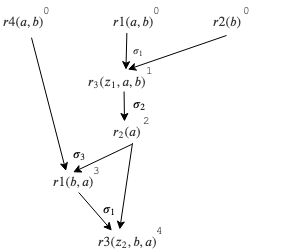
\includegraphics[scale=0.5]{chase_graph}
    \centering
    \caption{Chase Graph}
    \label{fig:chase_graph}
\end{figure}

Mostramos ahora, a modo de comparación el \textit{guarded chase forest}, para mismo $D$ y $\Sigma$. Notar que el mismo es un sub-grafo del anterior y que las profundidades de los nodos son ahora siempre menores o iguales que sus respectivos niveles de \textit{derivación} en el  \textit{chase graph}. 

\begin{figure}[ht]
    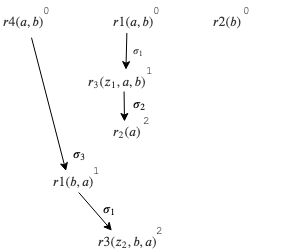
\includegraphics[scale=0.5]{guarded_chase_forest}
    \centering
    \caption{Guarded Forest}
    \label{fig:guarded_forest}
\end{figure}

\end{exmp}

\subsubsection{Bounded guard-depth property para el fragmento Guarded}

Sea $R$ un esquema relacional y $\Sigma$ un conjunto de TGDs para $R$. Decimos que $\Sigma$ tiene la propiedad \textit{Bounded guard-depth property} solo si, para toda base de datos $D$ y para toda consulta conjuntiva booleana $Q$, para toda vez que exista un homomorfismo $\mu$ que mapea $Q$ en el $chase(D, \Sigma)$, entonces existe un homomorfiso $\delta(Q)$ tal que todos los ancestros de $\delta(Q)$ en el $chase graph$ para $D$ y $\Sigma$ están contenidos en el $g-chase^{\gamma_k}(D, \Sigma)$, donde $\gamma_k$ solo depende de $Q$ y $R$.

Tal como se muestra en \cite{JWS}, las TGDs del fragmento Guarded poseen la propiedad anterior. En resumen, todos los átomos que se encuentran en la respuesta a una consulta conjuntiva se encuentran dentro del $g-chase^{(n + 1)\cdot\delta}$, con $\delta = (2\cdot\omega)^\omega\cdot2^{(2\omega)^{\omega\cdot|R|}}$, siendo $\omega$ la máxima aridad de algún predicado en $R$ y $n$ la cantidad de átomos en la consulta.

Esta profundidad en el \textit{guarded chase forest}, es independiente del tamaño de $D$, lo cual lleva a poder afirmar que responder consultas en el fragmento \textit{guarded} es $P-complete$ en la complejidad de datos.

\subsection{Datalog+/-, fragmento Lineal}

En el fragmento \textit{Lineal} de Datalog+/- las TGDs tienen un solo átomo en su cuerpo, es decir que tienen la forma $\forall X \forall  Y \Phi(X, Y) \rightarrow \exists Z \Psi(X,Z)$, siendo $\Phi(X,Y)$ un sólo átomo. Este fragmento esta estrictamente dentro del fragmento guarded, y aún perdiendo cierto poder expresivo con respecto al anterior, es lo suficientemente expresivo como para representar ontologías encodeadas en las \textit{Description Logics} de la familia \textit{Dl-Lite}. Además, tiene la ventaja de ser \textit{FO-rewritable} en la complejidad de datos.

\subsubsection{Bounded derivation-depth property}

Definimos ahora la \textit{bounded derivation-depth property} para un conjunto de TGDs, la cual es estrictamente más fuerte que la \textit{ bounded guard-depth property}, dado que la primera implica la segunda, pero no al revés. Informalmente, la \textit{bounded derivation-depth property} dice que para responder a una consulta conjuntiva no es necesario ir más allá de una profundidad $k$ en el \textit{chase graph} (y no en el \textit{guarded chase forest} como en el fragmento anterior), cuyo tamaño solo depende de $Q$ y $R$.

\subsubsection{First-order rewritability}
Una clase de TGDs $C$ es reescribible en primer orden o \textit{first-order rewritible} si solo si para todo conjunto de TGDs en $C$ y para toda consulta conjuntiva booleana $Q$, existe una consulta de primer orden $Q_\Sigma$ tal que, para toda base de datos $D$, sucede que $D \cup \Sigma \models Q$ si solo si $D \models Q_\Sigma$. Dado que responder consultas de primer orden es un problema en $AC_0$ en la complejidad de datos \cite{Vardi}, también se encuentra en esta clase de problemas responder consultas bajo TGDs que sean reescribibles en primer orden. Teniendo en cuenta además que toda consulta de primer orden es reescribible a una consulta $Q^*$ de \textit{SQL}, esta propiedad nos indica que para el fragmento \textit{lineal} podemos hacer uso práctico de los motores de base de datos \textit{SQL} con todas las optimizaciones ya provistas por los mismos.

\begin{figure}[ht]
    \includegraphics[scale=0.3]{fo_rewrite.jpg}
    \centering
    \caption{First Order Rewrite}
    \label{fig:fo_rewrite}
\end{figure}

\begin{exmp}\label{ejemplo_rewrite}
Consideremos el siguiente conjunto $\Sigma_T$ de TGDs en el fragmento \textit{lineal} sobre un esquema $R$:
    \begin{itemize}
        \item $\sigma_1 = bonaerense(X) \rightarrow argentino(X)$
        \item $\sigma_2 = cordob\acute{e}s(X) \rightarrow argentino(X)$
        \item $\sigma_3 = londinense(X) \rightarrow ingl\acute{e}s(X)$
        \item $\sigma_4 = casado(X) \rightarrow \exists Z casadoCon(X, Z)$
    \end{itemize}
Si tenemos $Q(X) = argentino(X) \land casadoCon(X, Z)$ podemos reescribir esta consulta como una unión de consultas en las que para cualquier base de datos $D$ sobre $R$, y sin tener en cuenta $\Sigma_T$, la unión de los resultados de tales consultas será el mismo que el resultado de $Q(X)$ sobre $D$ y $\Sigma_T$. Es fácil ver que en este caso, la unión de las siguientes consultas es una reescritura válida $Q(X)$ $\Sigma_T$:

    \begin{itemize}
        \item $Q_1(X) = argentino(X) \land casadoCon(X, Z)$
        \item $Q_2(X) = bonaerense(X) \land casadoCon(X, Z)$
        \item $Q_3(X) = cordob\acute{e}s(X) \land casadoCon(X, Z)$
        \item $Q_4(X) = argentino(X) \land casado(X)$
        \item $Q_5(X) = bonaerense(X) \land casado(X)$
        \item $Q_6(X) = cordob\acute{e}s(X) \land casado(X)$
    \end{itemize}
\end{exmp}

Se han propuesto diversos algoritmos de reescritura [\cite{Kewen}, \cite{Gottlob}]. El objetivo en este caso es conseguir una reescritura lo más chica posible, dado que esto permitirá un uso práctico real de los sistemas de base de datos \textit{SQL}. Si el resultado de la reescritura fuera una consulta demasiado grande, esto atentaría contra el uso práctico real, dado que los motores \textit{SQL} no muestran buena \textit{performance} para tales consultas. 

\subsection{Negative Constraints}\label{ncs}
Una \textit{Negative Constraint} es una fórmula de primer orden de la forma $\forall X \Phi (X) \rightarrow \bot$, donde $\Phi(X)$ es una conjunción de átomos. Estas \textit{constraints} nos ayudan a expresar restricciones sobre las ontologías.

\begin{exmp}
Podemos decir que los predicados esNegativo y esPositivo representan dos clases que no tienen instancias en común de la siguiente forma: $$esPositivo(X) \land esNegativo(X) \rightarrow \bot$$
De manera similar podemos decir que ningún miembro de una clase pertenece a una relación:$$soltero(X) \land casadoCon(X, Y) \rightarrow \bot $$ Podemos inclusive expresar que dos relaciones son disjuntas: $$mayor(X,Y) \land menor(X, Y) \rightarrow \bot$$
\end{exmp}

Responder consultas en una base de datos bajo un conjunto de TGDs $\Sigma_T$ y un conjunto de restricciones $\Sigma_C$ puede realizarse sin agregar complejidad de la siguiente manera: para cada \textit{negative constraint} $\sigma = \Phi(X,Y) \rightarrow \bot \in \Sigma_C$ verificamos que se satisface en $D$ y $\Sigma_T$, lo cual se puede hacer chequeando que la consulta conjuntiva booleana $Q_\sigma = \Phi(X, Y)$ evalúe a Falso en $D$ y $\Sigma_T$. Escribimos $D \cup \Sigma_T \models \Sigma_C$ si solo si toda $\sigma \in \Sigma_C$ es falsa en $D$ y $\Sigma_T$. Esto nos lleva inmediatamente al siguiente resultado: decimos que una consulta conjuntiva booleana es verdadera en $D$, $\Sigma_T$ y $\Sigma_C$, y lo anotamos $D \cup \Sigma_T \cup  \Sigma_C \models Q$ si solo si (i) $D \cup \Sigma_T \models Q$ o (ii) $D \cup \Sigma_T \not\models \Sigma_C$.

\subsection{Equality-Generating Dependencies (EGDs) y Keys}
Las dependencias generadoras de igualdad o \textit{Equality-Generating Dependencies} también son importantes a la hora de representar ontologías. Estas son fórmulas de primer orden que generalizas dependencias funcionales y en particular claves.

Sin embargo, si bien es cierto que agregar negative constraints es sencillo desde el punto de vista computacional, no sucede lo mismo con las EGDs: la interacción entre las TGDs y las EGDs puede tornar indecidible el problema de responder consultas\cite{Johnson}. Se puede comprobar que un conjunto fijo de EGDs y guarded TGDs pueden simular una maquina de Turing universal, con lo cual responder consultas es indecidible para tales dependencias. Por tal motivo, consideramos ahora una clase más restringida de EGDs, a las cuales llamamos \textit{claves no conflictivas}. Tal clase de EGDs muestra una interacción controlada con las TGDs (y NCs), de manera tal que no incrementan la complejidad de responder consultas, agregando al mismo tiempo suficiente poder expresivo para poder modelar ontologías.

Una \textit{dependencia generadora de igualdad} (o EGD) es una fórmula $\sigma$ de primer orden de la forma $\forall X \Phi(X) \rightarrow X_i = X_j$, donde $\Phi(X)$, el cual llamamos el cuerpo de $\sigma$, es una conjunción (no necesariamente guarded) de átomos, y $X_i$ y $X_j$ son variables en $X$. Llamamos a $X_i = X_j$ a la cabeza de $\sigma$. Tal $\sigma$ se satisface en una base de datos $D$ para $R$ si solo si, siempre que exista un homomorfismo $h$ tal que $h(\Phi(X) \subseteq D$, sucede que $h(X_i) = h(X_J)$. Se suelen omitir los cuantificadores universales en estas fórmulas, y consideramos solo conjuntos finitos de EGDs.

\begin{exmp}
La siguiente fórmula $\sigma$ es una EGD: $$r(X, Y_1) \land r(X,Y_2) \rightarrow Y_1 = Y_2.$$

La base de datos $D = \{r(a, b), r(c, d)\}$ satisface $\sigma$, dado que todo homomorfismo h que mapee el cuerpo de $\sigma$ a átomos de $D$ es tal que $h(Y_1) = h(Y_2)$. Por el contrario, la base de datos $D = \{r(a, b), r(a, d)\}$ no satisface $\sigma$.

\end{exmp}

Una EGD $\sigma$ sobre $R$ de la forma $\Phi(X) \rightarrow X_i = X_j$ es \textit{aplicable} a una base de datos $D$ si solo si existe un homorfismo $\eta : \Phi(X) \rightarrow D$ tal que $\eta(X_i)$ y $\eta(X_j)$ son distintos y no son ambos constantes. Si $\eta(X_i)$ y $\eta(X_j)$ son constantes distintas en $\Delta$, entonces hay una violación de $\sigma$, y el chase falla. Caso contrario, el resultado de aplicar $\sigma$ a $D$ es la base de datos $h(D)$ que se obtiene a partir de $D$ al reemplazar toda ocurrencia de algún elemento no constante $e https://www.overleaf.com/project/5d595ee258698f10f21f3b7a\in \{\eta(X_i), \eta(X_j)\}$ en $D$ para el otro elemento $e\prime$ (si $e$ y $e\prime$ son los dos nulos, entonces $e$ precede a $e\prime$ en orden lexicográfico.)

El chase para una base de datos $D$ y un conjunto $\Sigma_T$ de TGDs más un conjunto $\Sigma_E$ de $EGDs$, el cual llamamos \textit{full chase} y denotamos $chase(D, \Sigma_T \cup \Sigma_E)$, se computa de manera iterativa por medio de aplicar todas las EGDs que sean aplicables entre cada aplicación de cada TGD como se describió previamente.

\begin{exmp}
Consideremos el siguiente conjunto de TGDs y EGDs $\Sigma = \{\sigma_1, \sigma_2, \sigma_3\}$:

\begin{itemize}
    \item [$\sigma_1:$] $p(X) \rightarrow \exists Z s(X, Z)$
    \item [$\sigma_2:$] $s(X, Y), r(X)  \rightarrow X = Y$
    \item [$\sigma_3:$] $s(X, Y), s(X, Z) \rightarrow Y = Z$
\end{itemize}

Sea $D$ la base de datos $\{p(a), r(a), s(a, b)\}$. En el cómputo de $chase(D, \Sigma)$, primero aplicamos $\sigma_1$ y agregamos el átomo $s(a, z_1)$, donde $z_1$ es un nulo. Entonces, al aplicar $\sigma_2$ sobre $r(a)$ y $s(a, z_1)$ transformamos $s(a, z_1)$ en $s(a, a)$. Ahora $\sigma_3$ resulta aplicable sobre $s(a, a)$ y $s(a, b)$, pero al intentar igualar $a = b$ el \textit{chase} falla, pues hay una violación, dado que $a$ y $b$ son constantes distintas en $\Delta$.
\end{exmp}

\subsubsection{Separabilidad}
Sea $R$ un esquema relacional, y sean $\Sigma_T$ y $\Sigma_E$ dos conjuntos de TGDs y EGDs sobre $R$, respectivamente. Entonces, $\Sigma_E$ es separable de $\Sigma_T$ si solo si para toda base de datos $D$ sobre $R$, se cumplen las siguientes condiciones: 
\begin{itemize}
    \item  Si hay una violación de una EGD $\sigma \in \Sigma_E$ en $chase(D, \Sigma_T \cup \Sigma_E)$, entonces hay también una violación de $sigma$ en $D$.
    \item Si no hay violación de ninguna EGD $\sigma \in \Sigma_E$ entonces para toda connsulta $Q$, sucede que $chase(D, \Sigma_T \cup \Sigma_E) \models Q$ si solo si $chase(D, \Sigma_T) \models Q$.
\end{itemize}

Esto implica que agregar EGDs separables a un conjunto de TGDs no incrementa la complejiad de contestar consultas, tanto en el caso lineal como el el guarded. Esto es porque alcanza con evaluar si cada EGD se satisface en D, y si esto ocurre podemos entonces armar el chase con las TGDs solamente.

\subsubsection{Claves}
Dado un predicado relacional $p$ sobre un esquema relacional $R$ una clave $K$ sobre $p$ es un conjunto de posiciones para el cual sucede que para toda base de datos $D$ sobre $R$ no pueden existir dos \textit{hechos} en $D$ para $p$ tales que los dos hechos tengan los mismos valores en todas las posiciones de $K$ pero distintos valores en posiciones que no estén incluidas en $K$. 

\begin{exmp}
Sea $p$ el predicado binario \textit{padreDe} sobre un esquema relacional $R$, donde la primer posición indica el DNI de una persona y la segunda posición el DNI de su padre. Sea $k[1]$ una clave definida sobre \textit{padreDe}. Esto indica que no pueden existir dos átomos en $D$ con igual DNI en la primera posición y distinto DNI en la segunda posición, es decir que ninguna persona puede tener dos padres diferentes.
\end{exmp}

Podemos definir una clave a partir de un conjunto de EGDs.
\begin{exmp}
Sea $p$ un predicado ternario sobre un esquema relacional $R$. Sea $k[1]$ una clave para $p$. Podemos expresar esta clave por medio de dos EGDs:
\begin{itemize}
    \item $p(X, Y_1, Z_1) \land p(X, Y_2, Z_2) \rightarrow Y_1 = Y_2$.
    \item $p(X, Y_1, Z_1) \land p(X, Y_2, Z_2) \rightarrow Z_1 = Z_2$.
\end{itemize}
\end{exmp}


\subsubsection{Claves no conflictivas}
Sea $K$ una clave, y sea $\sigma$ una TGD de la forma $\Phi(X, Y) \rightarrow \exists Z r(X, Z)$. Decimos que $K$ es no conflictiva (NC) con $\sigma$ si se cumple alguna de las siguientes condiciones:
\begin{itemize}
    \item El predicado relacional sobre el cual $K$ está definido es diferente de $r$.
    \item Las posiciones de $K$ en $R$ no son un subconjunto propio de las posiciones de $X$ en $r$ en la cabeza de $\sigma$, y toda variable en $Z$ aparece una sola vez en la cabeza de $\sigma$. 
\end{itemize}

Decimos que $K$ es no conflictiva con un conjunto de TGDs $\Sigma_T$ si solo si $k$ es no conflictiva con toda $\sigma \in \Sigma_T$. Un conjunto de claves $\Sigma_K$ es no conflictivo con $\Sigma_T$ si solo si todas clave $k \in \Sigma_K$ es no conflictiva con $\Sigma_T$.

\begin{exmp}
Consideremos las siguientes claves $K_1, K_2, K_3, K_4$ definidas por los siguientes conjuntos de posiciones para el predicado $r$: $K_1=\{r[3]\}, K_2=\{r[2], r[3]\}, K_3=\{r[1]\},  K_4=\{r[1], r[2]\}$, y la TGD $\sigma = p(X, Y) \rightarrow \exists Z r(Z, X, Y)$. Teniendo en cuenta entonces que la cabeza de $\sigma$ es $r$, y el conjunto de posiciones en $r$ con variables cuantificada universalmente es $H = \{r[2], r[3]\}$, resulta que $K_1$ es la única clave definida por un conjunto de posiciones que es subconjunto propio de $H$. Por lo tanto salvo $K_1$, todas las claves son no conflictivas con $\sigma$.
\end{exmp}

Tal como se muestra en \cite{JWS}, la propiedad de no conflictivdad entre un conjunto de claves y un conjunto de TGDs, implica su separabilidad. La principal idea detrás de la prueba se describe a continuación. La condición de no conflictividad entre una clave $K$ y una TGD $\sigma$ asegura que o bien (a) la aplicación de $\sigma$ en el \textit{chase} genera un átomo con un nuevo nulo en una posición de $K$, y entonces este nuevo átomo no viola K; o bien (b) las posiciones cuantificadas universalmente en la cabeza de $\sigma$ coinciden con las posiciones de la clave $K$, con lo cual cualquier átomo nuevo generado a partir de $\sigma$ debe tener nulos frescos en todas las posiciones salvo las de la clave, no produciéndose una violación en este caso tampoco. Como todos los nuevos nulos son distintos entre sí, el \textit{chase} es homomórficamente equivalente al \textit{TGD full chase}.

Concluímos entonces esta sección afirmando que en el caso NC, las claves no incrementan la complejidad-datos de contestar consultas bajo TGDs y constraints, tanto para el fragmento \textit{guarded} como para el \textit{lineal}.

\subsection{Manejo de inconsistencia}
Durante mucho tiempo se ha estudiado el problema de manejar la inconsistencia en las bases de datos. En los últimos años, ha habido un creciente interés en este tema con el advenimiento de la \textit{Web Semántica}, que ha hecho que este asunto sea aún más relevante; teniendo en cuenta que en ambientes abiertos, con fuentes de información proveniente de diversos orígenes, es habitual que surjan contradicciones entre los datos.

Por otro lado, es bien sabido que la inconsistencia también genera problemas en la lógica clásica. En particular, las teorías lógicas inconsistentes no tienen modelos, y por lo tanto implican todas las fórmulas; con lo cual, responder consultas en una base de conocimientos inconsistente carece de sentido. Esto llevó a que en el campo de la inteligencia artificial y de la teoría de base de datos, se haya mantenido tradicionalmente la postura de que las bases de conocimiento deberían ser totalmente libres de información inconsistente, y que esta debería ser erradicada inmediatamente. Sin embargo, en las últimas décadas, se ha reconocido que para muchas aplicaciones interesantes aquella postura es obsoleta. 
Existen dos enfoques para lidiar con la inconsistencia. El primero consiste en que dada una base de conocimiento inconsistente, se debe arreglarla de una manera optimal. Esto puede implicar cambios en la teoría lógica subyacente tanto como agregar o quitar sentencias de la base. Este enfoque se caracteriza por tener una ``nocion coherentista'' en la que nos quedamos con una nueva base de datos que reemplaza a la original.  
El segundo enfoque se basa en considerar todas las maneras posibles de arreglar esa base de conocimientos \textit{on the fly}, es decir al momento de realizas las consultas. De alguna manera se ``convive'' con la inconsistencia. En este trabajo nos concentramos en este enfoque para el caso específico de teorías en \textit{Datalog +/-}. 
En lo que sigue describiremos distintas semánticas para \textit{query answering} tolerante a la inconsistencia. Todas ellas se basan en la noción de \textit{data base repair}. El objetivo es, a través de las consultas, obtener siempre información consistente; intentando a la vez alcanzar un buen equilibrio entre el poder expresivo de las semánticas y la complejidad computacional que estas requieren. 
\subsubsection{Inconsistencia en Datalog +/-}

Asumiremos en este trabajo que las \textit{TGDs, NCs y Keys} son correctas; es decir, capturan correctamente la semántica del dominio. Esta suposición implica que el conjunto $\Sigma$  dado por $\Sigma_T \cup \Sigma_N \cup \Sigma_K$  es siempre satisfacible; es decir que la aplicación de las TGDs no generan inconsistencias. En este enfoque los conflictos se generan a partir de los datos: la instancia de base de datos es la parte que debe ser \textit{reparada} o \textit{modificada} para restaurar la consistencia pudiendo así cumplir con las restricciones que impone el conjunto dado por $\Sigma_N \cup \Sigma_K$ . Cabe mencionar que esta no es la única opción. Muchos trabajos actuales se enfocan en otras posibilidades (\cite{Huang}, \cite{Hitzler}, \cite{Parsia}, \cite{Haasa}).

\subsubsection{Database repairs}

Mencionamos anteriormente que nuestro objetivo es obtener información consistente, aún conviviendo en ambientes con datos inconsistentes. ¿Pero como podemos obtener información consistente a partir de una base de datos que no lo es?. La principal herramienta que utilizaremos para alcanzar este objetivo es la noción de \textit{data base repair.} Dada una base de datos $D$ que contradice un conjunto de restricciones de integridad y de claves obtendremos un subconjunto de $D$ que no contradice estas restricciones pero que difiere de $D$ \textit{minimalmente}. Formalmente decimos que un \textit{repair} para ($D$, $\Sigma$) es una base de datos $D\prime$ tal que:
\begin{itemize}
    \item $D\prime \subseteq D$
    \item $mods(D\prime, \Sigma) \neq \varnothing $
    \item $\neg \exists D\prime \prime$ t.q. $D\prime\prime \subset D\prime \land mods(D\prime \prime, \Sigma) \neq \varnothing$
\end{itemize}

\begin{exmp}\label{ejemplo_ar}
Sea $R$ un esquema relacional y sea $\Sigma_T$ un conjunto de TGDs para $R$ dado por:
    \begin{itemize}
        \item $\sigma_1 = amigos(X, Y) \rightarrow tieneAmigos(X)$
        \item $\sigma_2 = amigos(X, Y) \rightarrow tieneAmigos(Y)$
        \item $\sigma_3 = amigos(X, Y) \land tienePiojos(X) \rightarrow tienePiojos(Y)$
    \end{itemize}
Sea $\Sigma_n$ el conjunto de restricciones dado por una única restricción
    \begin{itemize}
        \item $\sigma_n = pelado(X) \land tienePiojos(X) \rightarrow \bot$
    \end{itemize}
Sea $D$ una base de datos para $R$ dada por los siguiente hechos:
    \begin{itemize}
        \item tienePiojos('Federico')
        \item amigos('Federico', 'Miguel')
        \item amigos('Miguel', 'Pablo')
        \item esPelado('Pablo')
    \end{itemize}
Al aplicar el algoritmo del \textit{chase} sobre $D$ y $\Sigma_T$ obtenemos que:
\begin{gather*}
    chase(D, \Sigma_T) = D \cup \{tieneAmigos('Federico'), tieneAmigos('Miguel'),\\ tieneAmigos('Pablo'), tienePiojos('Miguel'), tienePiojos('Pablo')\}
\end{gather*}

Vemos entonces que en $chase(D, \Sigma_T)$ hay una violación de $sigma_n$, pues resulta que este contiene simultáneamente los átomos $esPelado('Pablo')$ y $tienePiojos('Pablo')$.
El conjunto de \textit{repairs} para $(D, \Sigma)$ está dado entonces por:
    \begin{itemize}
        \item $r_1 = \{ tienePiojos('Federico'), amigos('Federico', 'Miguel'), amigos('Miguel', 'Pablo')\}$
        \item $r_2 = \{ tienePiojos('Federico'), amigos('Federico', 'Miguel'), esPelado('Pablo')\}$
        \item $r_3 = \{ tienePiojos('Federico'), amigos('Miguel', 'Pablo'), esPelado('Pablo')\}$
        \item $r_4 = \{ amigos('Federico', 'Miguel'), amigos('Miguel', 'Pablo'), esPelado('Pablo')\}$
    \end{itemize}
    
Notar que en este caso cada uno de los \textit{repairs} está dado por incluír en el \textit{repair} cualquier subconjunto de tres átomos de entre los cuatro átomos de $D$. Al decir que Federico es amigo de Miguel, y que Miguel es amigo de Pablo, y al decir que los amigos se contagian los piojos, tiene que ser que Federico le contagio los piojos a Miguel y este se los contagió a Pablo. Pero esto no puede ser porque Pablo es pelado. Observar entonces que quitando cualquier átomo de $D$, obtenemos un subconjunto maximal consistente.
    
\end{exmp}

\subsubsection{Semántica AR}
La semántica AR, es la más aceptada para \textit{query answering} en ontologías potencialmente inconsistentes. Dada una base de conocimiento $(D, \Sigma)$ y una consulta conjuntiva $Q$, decimos que $(D, \Sigma) \models_{AR} Q$ si solo si $(R, \Sigma) \models Q$ para todo R \textit{repair} de $(D, \Sigma)$.

En el ejemplo anterior, si tomamos $Q() = tieneAmigos('Miguel')$, resulta que $(D, \Sigma) \models_{AR} Q$. En cambio, si consideramos la consulta $Q() = tieneAmigos('Pablo')$ resulta que $(D, \Sigma)\not\models_{AR} Q$.

\tituloTesis{}La semántica AR definida arriba coincide con la semántica tolerante a la inconsistencia para Lógicas de Descripción presentada en \cite{Lembo}. Aunque esta semántica puede ser considerada en cierto sentido la elección natural para el objetivo semántico que estamos buscando, tiene la desventaja de ser dependiente de la forma sintáctica de la base de conocimiento. Supongamos que la base de conocimiento $KB\prime = (D\prime, \Sigma)$ difiere de la base de conocimiento $KB = (D, \Sigma)$ simplemente porque $D\prime$ incluye átomos que se pueden inferir a partir de $\Sigma$ y un subconjunto consistente de $D$. En este caso $KB$ y $KB\prime$ son lógicamente equivalentes, y cabe esperar por lo tanto que sus \textit{repairs} coincidan y que las respuestas a toda consulta sobre $KB$ y $KB\prime$ coincidan bajo toda semántica. Sin embargo esto no sucede con la semántica \textit{AR}. 


\begin{exmp}\label{ejemplo_ar_2}
Considerando $D$ y $\Sigma$ del ejemplo anterior, definamos ahora la base de datos $D\prime$ dada por $D \cup \{tieneAmigos('Pablo')\}$. Es claro que el nuevo átomo introducido se puede inferir lógicamente de $D$ y $\Sigma$, notar de hecho que el mismo se encuentra en el chase de aquel ejemplo. Si consideramos ahora los \textit{repairs} para $D\prime$ y $\Sigma$ obtenemos
    \begin{itemize}
        \item $r\prime_1 = r_1 \cup \{tieneAmigos('Pablo')\}$
        \item $r\prime_2 = r_2 \cup \{tieneAmigos('Pablo')\}$
        \item $r\prime_3 = r_3 \cup \{tieneAmigos('Pablo')\}$
        \item $r\prime_4 = r_4 \cup \{tieneAmigos('Pablo')\}$
    \end{itemize}

Con lo cual resulta que $(D\prime, \Sigma)\models_{AR} tieneAmigos('Pablo')$, resultado opuesto para la $KB$ del ejemplo anterior.
\end{exmp}

\subsubsection{Semántica CAR}
Dependiendo del escenario particular en el que se quiera resolver este tipo de inconsistencias, el comportamiento anterior podría ser considerado incorrecto. Esto motivó la definición de una nueva semántica que no presenta esta característica. De acuerdo con esta semántica, llamada \textit{Closed ABox Repair}, los \textit{repairs} toman en cuenta no solo los hechos explícitamente incluídos en $D$, sino también aquellos hechos que se pueden inferir junto con $\Sigma$ y al menos un subconjunto de $D$ que sea consistente.
Para formalizar la idea anterior, es necesario dar primero las siguientes definiciones. Dada una base de conocimiento $K = (D, \Sigma)$, denotamos por medio de $HB(K)$ a la \textit{Herbrand Base} de $K$, es decir el conjunto de hechos que se pueden construir sobre el alfabeto de de $\Gamma_K$. Definimos después las consecuencias lógicas de $K$ como el conjunto $clc(K) = \{\alpha | \alpha \in HB(K) \land \exists S \subseteq D$ tal que $Mods(S, \Sigma) \neq  \varnothing \land (S, \Sigma) \models \alpha \}$. Podemos ahora dar la siguiente definición de \textit{Closed ABox Repair}.

Sea $K = (D, \Sigma)$ una base de conocimiento en Datalog+/-. Un \textit{Car Repair} de $K$ es un conjunto $D\prime$ de hechos tales que:
    \begin{enumerate}
        \item $D\prime \subseteq clc(K)$
        \item $mods(D\prime, \Sigma) \neq \varnothing$
        \item $\neg\exists D\prime\prime$ tal que $mods(D\prime\prime, \Sigma) \neq \varnothing$ y :
        \begin{itemize}
            \item $D\prime\prime \cap D \supset D\prime \cap D$ o,
            \item $D\prime\prime \cap D = D\prime \cap D \land D\prime\prime \supset D\prime$   
        \end{itemize}
    \end{enumerate}

Denotamos por medio de $CAR-Rep(D, \Sigma)$ al conjunto de todos los \textit{Car Repairs} para $K$.
Intuitavemnte, un \textit{CAR-repair} es un subconjunto de \textit{clc(K)} consistente con $\Sigma$ que preserva máximamente al conjunto de hechos $D$. En particular, la condición 3 dice que preferimos a $D\prime$ por encima de cualquier otro $D_R \subseteq clc(K)$ consistente con $\Sigma$ tal que $D_R \cap D \subset D\prime \cap D$ (es decir que $D_R$ mantiene un subconjunto más pequeño de $D$ con respecto a $D\prime$). Entonces, entre todos aquellos subconjuntos $D_R$ que tengan la misma intersección con $D$, preferimos a aquellos que contengan la mayor cantidad de hechos en \textit{clc(K)} posibles.
Dada $KB = (D, \Sigma)$ y una consulta conjuntiva $Q$, decimos que $KB \models_{CAR} Q$ si solo si $(R, \Sigma) \models Q$ para cada $R \in CAR-Rep(D, \Sigma)$.

\begin{exmp}\label{ejemplo_car_repairs}
Consideremos las bases de conocimiento presentadas en \ref{ejemplo_ar} y en el \ref{ejemplo_ar_2} y veamos que en este caso el conjunto de \textit{CAR-repairs} es el mismo para las dos bases. Para eso construímos primero el conjunto \textit{clc(K)}. Es fácil ver que para ambos ejemplos este conjunto esta dado por clc(K) = \{amigos('Federico', 'Miguel'), amigos('Miguel', 'Pablo'), tieneAmigos('Federico'), tieneAmigos('Miguel'), tieneAmigos('Pablo'), tienePiojos('Federico'), tienePiojos('Miguel'), tienePiojos('Pablo'), esPelado('Pablo')\} y que en ambos casos el conjunto de \textit{CAR-repairs} está dado por:
        \begin{itemize}
            \item \{amigos('Federico', 'Miguel'), amigos('Miguel', 'Pablo'), tieneAmigos('Federico'), tieneAmigos('Miguel'), tieneAmigos('Pablo'), tienePiojos('Federico'), tienePiojos('Miguel'), tienePiojos('Pablo')\}
            \item \{amigos('Federico', 'Miguel'), amigos('Miguel', 'Pablo'), tieneAmigos('Federico'), tieneAmigos('Miguel'), tieneAmigos('Pablo'),  esPelado('Pablo')\}
            \item \{amigos('Federico', 'Miguel'), tieneAmigos('Federico'), tieneAmigos('Miguel'), tieneAmigos('Pablo'), tienePiojos('Federico'), tienePiojos('Miguel'),  esPelado('Pablo')\}
           \item \{amigos('Miguel', 'Pablo'), tieneAmigos('Federico'), tieneAmigos('Miguel'), tieneAmigos('Pablo'), tienePiojos('Federico'), esPelado('Pablo')\}
        \end{itemize}
Notar que dado que el conjunto de \textit{CAR-repairs} es el mismo para ambas bases de conocimiento, las respuestas serán siempre las mismas para toda consulta $Q$ bajo esta semántica. En particular teniendo en cuenta $D$ y $\Sigma$ del ejemplo \ref{ejemplo_ar} tenemos que $$(D, \Sigma)\models_{CAR} tieneAmigos('Pablo'),$$ y lo mismo ocurre para $D\prime$ y $\Sigma$ del ejemplo \ref{ejemplo_ar_2}.
\end{exmp}

\subsubsection{Semánticas de intersección}
En general, responder consultas es intratable tanto para la semántica \textit{CAR} como \textit{AR}. Dado que esto supone un obstáculo en su uso práctico, se propusieron aproximaciones de estas semánticas, para las cuales se ha demostrado que responder consultas conjuntivas es polinomial en las lógicas de descripción \textit{DL-Lite}. En ambos casos, la aproximación consiste en tomar como único \textit{repair} la intersección de los \textit{AR-repairs} y de los \textit{CAR-repairs} respectivamente. Esta idea se corresponde con el enfoque \textit{WIDTIO (When you are in doubt throw it out)}, provenitente del área de revisión de creencias [\cite{Eiter},\cite{Winslett}].

\subsubsection{Semántica IAR}
Sea $KB = (D, \Sigma)$ una base de conocimiento, y sea $Q$ una consulta conjuntiva. Decimos que $KB \models_{IAR}$ si solo si $(\cap_{R \in AR-Rep(D, \Sigma)}, \Sigma)\models Q$ 

\begin{exmp}\label{ejemplo_iar}
Consideremos $(D, \Sigma)$ y el conjunto de \textit{AR-repairs} del ejemplo \ref{ejemplo_ar}. La intersección de aquellos \textit{repairs} es el conjunto vacío. Por lo tanto, para toda consulta $Q$ resulta que $(D, \Sigma)\not\models_{IAR} Q$. Si consideramos en cambio $(D\prime, \Sigma)$ del ejemplo \ref{ejemplo_ar_2} y consideramos la consulta $Q() = tieneAmigos('Pablo')$, resulta que $(D, \Sigma)\models_{IAR} Q$. Notar entonces que la semántica \textit{IAR} sufre la misma desventaja que la semántica \textit{AR}, pues también es dependiente de la forma sintáctica de la base de conocimiento.
\end{exmp}

\subsubsection{Semántica ICAR}
De manera análoga a la definición de la semántica \textit{IAR} definimos la semántiuca \textit{ICAR}. Sea $KB = (D, \Sigma)$ una base de conocimiento, y sea $Q$ una consulta conjuntiva. Decimos que $KB \models_{ICAR}$ si solo si $(\cap_{R \in CAR-Rep(D, \Sigma)}, \Sigma)\models Q$

\begin{exmp}
Al igual que la semántica \textit{CAR}, la semántica \textit{ICAR} tiene la ventaja de no ser dependiente de la forma sintáctica de la KB. Teniendo en cuenta lo comentado en el ejemplo \ref{ejemplo_car_repairs}, es fácil ver que tanto para la base de conocimiento presentada en el ejemplo \ref{ejemplo_ar} como para la presentada en el ejemplo \ref{ejemplo_ar_2}, la intersección de los \textit{CAR-repairs} coincide. Esta intersección está dada por el conjunto \{tieneAmigos('Federico'), tieneAmigos('Miguel'), tieneAmigos('Pablo')\}. Podemos ejemplificar entonces diciendo que:
\begin{itemize}
    \item $(D, \Sigma) \models_{ICAR} tieneAmigos('Pablo')$.
    \item $(D, \Sigma) \not\models_{ICAR} sonAmigos('Miguel','Pablo')$.
\end{itemize}

\end{exmp}

\subsubsection{Semántica ICR}
Sea $Cn(D,\Sigma)$ la clausura lógica de $D$ y $\Sigma$. Sea $KB$ una base de conocimiento $(D, \Sigma)$, y sea $Q$ una consulta conjuntiva. Decimos que $KB \models_{ICR} Q $ si solo si $(\cap_{R \in Rep(KB)}, Cn(R, \Sigma))\models Q$. Veremos a continuación que esta semántica es una \textit{aproximación \textit{sana}} de \textit{AR} e \textit{ICAR}, y que además es una aproximación \textit{completa} de \textit{IAR}.

\begin{exmp}
Consideremos $D$ y $\Sigma$ del ejemplo \ref{ejemplo_ar}. Tenemos que calcular las clausuras lógicas de los cuatro \textit{repairs} de ese mismo ejemplo.
    \begin{itemize}
        \item $Cn(r_1)$ = \{ tienePiojos('Federico'), amigos('Federico', 'Miguel'), amigos('Miguel', 'Pablo'), tienePiojos('Miguel'), tienePiojos('Pablo'), tieneAmigos('Federico'), tieneAmigos('Miguel'), tieneAmigos('Pablo')\}
        \item $Cn(r_2)$ = \{ tienePiojos('Federico'), amigos('Federico', 'Miguel'), esPelado('Pablo'), tieneAmigos('Federico'), tieneAmigos('Miguel'), tienePiojos('Miguel')\}
        \item $Cn(r_3)$ = \{ tienePiojos('Federico'), amigos('Miguel', 'Pablo'), esPelado('Pablo'), tieneAmigos('Miguel'), tieneAmigos('Pablo')\}
        \item $Cn(r_4)$ = \{ amigos('Federico', 'Miguel'), amigos('Miguel', 'Pablo'), esPelado('Pablo'), tieneAmigos('Federico'), tieneAmigos('Miguel'), tieneAmigos('Pablo') \}
    \end{itemize}
La intersección de estos conjuntos esta dada por \{ tieneAmigos('Federico'), tieneAmigos('Miguel') \}. Podemos decir entonces que $(D, \Sigma) \models_{ICR} tieneAmigos('Federico') \land tieneAmigos('Miguel')$.
\end{exmp}
Notemos que tal como se comentó en el ejemplo \ref{ejemplo_iar}, para mismo $D$ y $\Sigma$, la intersección de los \textit{repairs} fue el conjunto vacío. Es decir que al menos en este caso la semántica \textit{IAR} fue más restrictiva que la semántica \textit{ICR}. Veremos en la próxima sección que en verdad esto se cumple para todo $D$ y todo $\Sigma$.

\subsection{Aproximaciones sanas y completas}
Dadas dos semánticas \textit{A} y \textit{B}, decimos que la semántica \textit{A} es \textit{sana} con respecto a la semántica \textit{B} si solo si para toda consulta $Q$ resulta que si Q es verdadera bajo la semántica \textit{A} también lo es bajo la semántica \textit{B}. Por el contrario, \textit{A} es \textit{completa} con respecto a \textit{B} si solo si para toda consulta $Q$ resulta que si $Q$ es verdadera bajo \textit{B} también lo es bajo \textit{A}. De esto se desprende que si \textit{A} es \textit{sana} respecto de \textit{B} entonces \textit{B} es \textit{completa} respecto de \textit{A}.

Veamos ahora como se aproximan entre sí las semánticas que hemos mencionado. En la siguiente figura hay una flecha que parte desde la semántica \textit{A} hacia la semántica \textit{B} si solo si la semántica \textit{A} es una aproximación sana de la semántica \textit{B}.


\begin{figure}[ht]
    \includegraphics[scale=0.3]{aproximaciones_sanas.png}
    \centering
    \caption{Aproximaciones entre las semánticas}
    \label{fig:aproximaciones}
\end{figure}

Tal como se muestra en el gráfico, \textit{IAR} es la semántica más restrictiva, siendo esta una aproximación \textit{sana} de \textit{ICR}, y siendo esta última una aproximación \textit{sana} de \textit{AR} e \textit{ICAR}, aunque estas dos no se aproximan entre sí. Por otro lado \textit{AR} e \textit{ICAR} son aproximaciones \textit{sanas} de \textit{CAR}, la menos restrictiva de todas las semánticas. 

\chapter{Resultados Formales}

\subsection{Algoritmo para encontrar los Repairs}
Presentamos en esta secci'on un algoritmo que dada una base de conocimientos $(D, \Sigma)$, con $\Sigma = \Sigma_T \cup \Sigma_N$, retorna todos sus \textit{repairs}, es decir todos los subconjuntos de $D$ maximales consistentes con respecto a $\Sigma$. Nuestro objetivo es recorrer la menor cantidad de subconjuntos de $D$ posibles.
Sea $n$ la cardinalidad del conjunto $D$, el algoritmo \textit{naive} consiste en armar los $2^n$ subconjuntos de $D$ y para cada uno de ellos evaluar cada una de las \textit{Negstive Constraints} en $\Sigma_N$, y en caso de que alguna fuera violada, decimos que el subconjunto no es consistente. Como explicamos en la sección \ref{ncs}, para evaluar una $NC: \phi(x, y) \rightarrow \bot$, podemos evalular la consulta $Q(X, Y) = \phi(X, Y)$ sobre $(D, \Sigma_T)$ y si la respuesta es distina al conjunto vacío entonces decimos hay una violación de tal \textit{NC}.

\subsection{Algoritmo RepairFinder}

Presentamos ahora un algoritmo que intenta minimizar el espacio de búsqueda y la cantidad de consultas a la base de conocimiento. 


\begin{algorithm}[H]
\SetAlgoLined
    \KwIn{$(D, \Sigma)$ }
    \KwOut{Repairs para $(D, \Sigma)$ }

$top \gets todosLosSubConjuntosDeUnElementoMenos(D)$\;
$bottom \gets todosLosSubConjuntosDeUnElemento(D)$\;
$culprits \gets \emptyset$\;
$repairsChicos \gets \emptyset$\;
$repairsGrandes \gets \emptyset$\;
$bottomMasUno \gets \emptyset $\;

\For{$s \in bottom$}{
$s.consistente \gets chequearConsistencia(s, \Sigma)$\;
\lIf{$\neg s.consitente$}{
$culprits.agregar(s)$}
}
$bottom \gets bottom.filtrarPor(s \Rightarrow s.consistente )$


 \While{top $\neq \emptyset$ {\bf and} bottom $\neq \emptyset$ {\bf and} top.any.size $>$ bottom.any.size   }{
            $ActualizarTop()$\;			
			$ActualizarBottom()$\;
}
 \caption{RepairFinder}
\end{algorithm}


\begin{algorithm}[H]
\SetAlgoLined
    \KwIn{$(D, \Sigma)$ }
\For{$s \in top$}{
     \lIf{$culprits.algunoCumple(c \Rightarrow c \subset s)$}{$s.consistente \gets false$}
     \Else{$s.consistente \gets chequearConsistencia(s, \Sigma)$\;
        \lIf{s.consistente}{repairsGrandes.agregar(s)}
        }
}

$topInconsistentes \gets top.filtrarPor(s \rightarrow s.consistente)$\;
$unionInconsistentes \gets ordenar(sinRepetidos(concatenar(topInconsistentes)))$\;
$proximoTop \gets subcojuntosDeTama\tilde{n}oTopMenosUno(unionInconsistentes)$\;

$top \gets proximoTop.filtrarPor(s \rightarrow topInconsistentes.algunoCumple(t \rightarrow s \subset t$  {\bf and} $repairsGrandes.ningunoCumple(r \rightarrow s \subset r) )) $
		

 \caption{ActualizarTop}
 
 
\end{algorithm}

\begin{algorithm}[H]
\SetAlgoLined
    \KwIn{$(D, \Sigma)$ }


 $proximoBottom \gets subcojuntosDeTama\tilde{n}oBottomMasUno(D)$\;
 $proximoBottom \gets proximoBottom.filtrarPor(s \rightarrow bottom.algunoCumple(b \rightarrow b \subset s$ {\bf and}  $culprits.ningunoCumple(c \rightarrow c \subset s)))$\;
\For{$s \in proximoBottom$}{
     \lIf{$repairsGrandes.algunoCumple(r \rightarrow s \subset r)$}{$s.consistente \gets true$}
     \Else{$s.consistente \gets chequearConsistencia(s, \Sigma)$\;
        \lIf{$\neg s.consistente$}{$culprits.agregar(s)$}
        }
}

\For{$s \in bottom$}{
     \If{$proximoBottom.filtrarPor(t \rightarrow s \subset t).todosCumplen(t \rightarrow \neg t.consistente) $}
        {$repairsChicos.agregar(s)$}
}
$bottom \gets proximoBottom.filtrarPor(s \rightarrow s.consistente)$\;

 \caption{ActualizarBottom}

\end{algorithm}


	para todos los s en bottom consistentes cuyos padres son todos inconsistentes //esto lo miro rapido gracias al grafo
		agregar s a repairsChicos


	para cada s en bottomMasUno:
		si s es subConbj de un repairGrande
			s.consistentStatus = consistent
		si no:
			tirar query y fijarse si es consistnete
			si s es consistente:
				s.consistentSatus = consistente
			si no
				s.consistentSatus = inconsistent
				agregar s a culprit. (esto lo puiedo hacer porque todos sus sub conjuntos
				son consistentes. por el absurdo: si alguno no lo fuera entonces 
				ese sub conjunto o bien es un culprit o bien es super conjunto de un culprit).















input: program

var top = todosLosSubSetDeUnoMenos(program.Abox);
var bottom = todosLosSetDeUnElemento(program.Abox);
var minimalesIncosistentes = vacio;
var repairsChicos = vacio;
var repairsGrandes = vacio;
var topMenos1 = vacio;
var bottomMasUno = vacio;

para cada s en bottom:
	fijarase si es consistente o no
	si s es inconsistente:
		s.consistentStatus = inconsistent
		agregar s a culprits
	si no:
		s.consistent = true
	
	bottom := bottom.filter(s -> s.consistents);

while(top != vacio and bottom != vacio and (top.get(0).Facts.size() > bottom.get(0).Facts.size() )  ){
			
	para cada set s en top:
	si s es superCojunto de un minimalInconsistente:
		s.consistentStatus = inconsistent		
			
	para cada s en top con consistentStatus en undefined: 
		fijarse si s es consistente (tirando las queries).
		si s es consistente: 
			s.consistent = true.
			agregar s a repairsGrandes// no hace falta mirar que no sea subconjutno de algun 
									//	repair grande existente, 
									//pues eso lo filtro cuando elijo los hijos de topMenos1
		si no
			s.consistente = false. //no necesariamente es inconsistente minimal.
	
	topMenosUno := todos los subSet que puedo generar sacando un elemento a 
				los set de top inconsistentes. filtrar solo a los que no sean 
				sub conjunto de un repair grande.
	.
	top = topMenosUno

	bottomMasUno = todos los subset de la ABox que se pueden formar agregnado un elemento 
				de la ABox a los consistentes.
				filtrar solo a los que no sean superConjunto de un minimal inconsistente. 
				
	//ir armando el grafo (hijo-padre). // el objeto AboxSubSet, donde cada uno tiene una lista de hijos y de padres

	
	para cada s en bottomMasUno:
		si s es subConbj de un repairGrande
			s.consistentStatus = consistent
		si no:
			tirar query y fijarse si es consistnete
			si s es consistente:
				s.consistentSatus = consistente
			si no
				s.consistentSatus = inconsistent
				agregar s a culprit. (esto lo puiedo hacer porque todos sus sub conjuntos
				son consistentes. por el absurdo: si alguno no lo fuera entonces 
				ese sub conjunto o bien es un culprit o bien es super conjunto de un culprit).
				
	para todos los s en bottom consistentes cuyos padres son todos inconsistentes //esto lo miro rapido gracias al grafo
		agregar s a repairsChicos
	
	bottom = bottomMasUno que sean consistentes
}

if (n es par) para cada s en topMenosUno: si es superconj de minimal  consistente: nada
	si no tirar query, si da consistente, agregarlo a maximal consistente





return {repairs: repairsChicos U repairsGrandes, intersection : intersection(this.repairs) }*/








INVARIANTE antes de arrancar el cuerpo de cada while:

TOP: 
	no se si son o no consistentes. 
	no son subconjuntos de ningun big repair. -> significa que si fueran consistentes serian 
	repairs, pues todos sus super conjuntos son inconsistentes. por el absurdo: su algun 
	superconjunto fuera consistente entonces o bien es un repair o bien es hijo de un repair.
	
Bottom:
	son consistentes.

Small Repairs:
	Todos los repairs de tamaño menor que los bottom ya fueron agregados a Small Repairs.

Culprits: 
	Todos los culprits de tamaño igual o menor que bottom ya fueron agregados a Culprits.

Big Repairs:
	Todos los repairs de mayor tamaño que top ya fueron agregados a Big Repairs.
	

	
	











%% ...

\chapter{Implementación}

%%%% BIBLIOGRAFIA
\backmatter
\begin{thebibliography}{9}
    \bibitem{beeri} 
    C. Beeri y M. Y. Vardi.
    \textit{The implication problem for data dependencies}. 
    En \textit{Proc. ICALP-1981}, pp. 73–85, 1981.
     
    \bibitem{cali} 
    A. Calı, G. Gottlob, y M. Kifer.
    Taming the infinite chase: Query answering under expressive relational constraints.
    En \textit{Proc. KR-2008, pp. 70–80, 2008}. 

    \bibitem{Chandra} 
    A. K. Chandra and P. M. Merlin. 
    Optimal implementation of conjunctive queries in relational data bases.
    En \textit{Proc. KR-2008, pp. 70–80, 2008}. 

    \bibitem{Deutsch} 
    A. Deutsch, A. Nash, and J. B. Remmel.
    The chase revisited.
    En \textit{Proc. PODS-2008, pp. 149–158, 2008}. 

    \bibitem{Fagin} 
    R. Fagin, P. G. Kolaitis, R. J. Miller, and L. Popa.
    Data exchange: Semantics and query answering.
    En \textit{Theor. Comput. Sci., 336(1):89–124, 2005.}. 

    \bibitem{Johnson} 
    D. S. Johnson and A. C. Klug.
    Testing containment of conjunctive queries under functional and inclusion dependencies.
    En \textit{J. Comput. Syst. Sci., 28(1):167–189, 1984}. 

    \bibitem{Vardi} 
    M. Y. Vardi
    On the complexity of bounded-variable queries.
    En \textit{Proc. PODS-1995, pp. 266–176, 1995}. 
    
    \bibitem{JWS} 
    Andrea Calì, Georg Gottlobc, Thomas Lukasiewicz.
    A General Datalog-Based Framework for Tractable Query Answering over Ontologies
    En \textit{QUE PONGO ACA}. 
    
    \bibitem{Huang} 
    Z. Huang, F. van Harmelen, and A. ten Teije.
    Reasoning with inconsistent ontologies.
    En \textit{Proc. of IJCAI 2005, pages 454–459, 2003}. 
    
    \bibitem{Hitzler} 
    Y. Ma and P. Hitzler.
    Paraconsistent reasoning for owl 2.
    En \textit{Proc. of RR 2009, pages 197–211, 2009.} 
    
    \bibitem{Parsia} 
    B. Parsia, E. Sirin, and A. Kalyanpur.
    Debugging OWL ontologies.
    En \textit{Proc. of WWW 2005, pages 633–640, 2005.} 

    \bibitem{Haasa} 
    P. Haasa, F. van Harmelen, Z. Huang, H. Stuckenschmidt, y Y. Sure.
    A framework for handling inconsistency in changing ontologies.
    En \textit{Proc. of ISWC 2005, 2005.} 

    \bibitem{Lembo} 
    D. Lembo and M. Ruzzi.
    Consistent query answering over description logic ontologies.
    En \textit{Proc. of RR 2007, 2007.} 
    
    \bibitem{Eiter} 
    T. Eiter and G. Gottlob.
    On the complexity of propositional knowledge base revision, updates and counterfactuals.
    En \textit{Artificial Intelligence, 57:227–270, 1992.} 
    
    \bibitem{Winslett} 
    M. Winslett.
    Updating Logical Databases.
    En \textit{Cambridge University Press, 1990} 
    
    \bibitem{Kewen} 
    Zhe Wang, Peng Xiao, and Kewen Wang.
    Practical Datalog Rewriting for Existential Rules
    En \textit{Griffith University, Australia} 
    
    \bibitem{Gottlob} 
    Georg Gottlob, Giorgio Orsi, and Andreas Pieris.
    Ontological Queries: Rewriting and Optimization
    En \textit{Department of Computer Science, University of Oxford. Oxford-Man Institute of Quantitative Finance, University of Oxford, UK. Institute for the Future of Computing, University of Oxford, UK } 





    \end{thebibliography}

\end{document}
